\section{Grundlagen}\label{sec:grundlagen}

% Es beginnt mit einem naiven Ansatz zur Optimierung von Ausdrücken und leitet zu \textit{E-Graphs} und \textit{Equality Saturation} über.

Dieses Kapitel leitet mit einem naiven Ansatz zur Optimierung ein und diskutiert die daraus entstehenden Nachteile.
Danach wir schrittweise zu \textit{E-Graphs}
übergeleitet und schließlich der Prozess \textit{Equality Saturation} erklärt.
Die folgenden beiden Abschnitte~\ref{subsec:naiv} und~\ref{subsec:egraphs} stützen sich auf~\cite{cole}. Viele Beispiele wurden aus dieser Quelle übernommen.

\subsection{Naives Optimieren}\label{subsec:naiv}

Für das naive Optimieren von Ausdrücken wird zuerst das Konzept der \textit{rewrite rules} benötigt. Gegeben sei ein beliebiger mathematischer Ausdruck, z.B.
$a * 1$. Um eine Umformung dieses Ausdrucks durchführen zu können, kann eine \textit{rewrite rule} auf diesen Ausdruck angewendet werden.
Als Beispiel sei hier die folgende Regel gegeben: $[\mathbf{1}]: x * 1 \Leftrightarrow x$. Die \textit{rewrite rule} besteht aus einem linken und rechten Teil. Der linke Teil
beschreibt ein \textbf{Muster}, das dem Ausdruck entsprechen muss. Das wird als \textit{Matching} bezeichnet. Dabei spielt der Name der Variablen, in diesem Falle $x$, keine Rolle.
Der rechte Teil vermittelt, in welche neue Form dieses Muster gebracht werden soll. Wendet man also Regel $[1]$ an,
ergibt sich: $a * 1  \overset{[2]}{\rightarrow} a$. 
Eine Regel wie $\frac{x}{x} \Leftrightarrow 1$ \textit{matcht} nicht und würde damit auch nicht angewendet werden können.
Mit diesen Bausteinen kann bereits ein naiver Algorithmus entworfen werden, der in Ansatz~\ref{alg:ausdruck1} skizziert wurde. 

% Gegeben sei ein mathematischer Ausdruck, zum Beispiel: $a * 1$. Um diesen Ausdruck umzuformen, kann eine \textit{rewrite rule} eingesetzt werden.
% Eine \textit{rewrite rule} beschreibt die Umformung eines Ausdrucks in einen anderen. Als Beispiel sei hier folgende Regel gegeben: $x * 1 \Leftrightarrow x \;\; (1)$.
% Angewendet auf den obigen Ausdruck würde sich folgendes ergeben: $a * 1  \overset{(1)}{\Leftrightarrow} a$.

% Die Anwendung dieser \textit{rewrite rule} ist nur möglich, weil die Regel \textit{matcht}. Das bedeutet, dass der Ausdruck und die linke Seite der Regel identisch sind 
% (abgesehen vom Namen der Variablen). Die folgende \textit{rewrite rule} würde nicht \textit{matchen} und damit auch nicht angewendet werden können: $\frac{x}{x} \Leftrightarrow 1$.
% Mit diesen Bausteinen lässt sich bereits ein naiver Algorithmus anfertigen, der in Abbildung~\ref{alg:ausdruck1} dargestellt ist.

\begin{algorithm}[H]
  \caption{Naiver Algorithmus zur Optimierung von Ausdrücken}\label{alg:ausdruck1}
  \begin{algorithmic}
    \Function{optimize\_expression}{expression}
    \State rules $\gets$ [\ldots]
    
    \While{old\_expression $\neq$ expression}
      \State old\_expression $\gets$ expression

      \For{rule in rules}
        \If{match(expression, rule)}
        \State apply(expression, rule)
        \EndIf
      \EndFor
    \EndWhile

    \State \Return expression
    \EndFunction
  \end{algorithmic}
\end{algorithm}

Der Algorithmus durchläuft solange die while-Schleife, bis keine Änderungen am Ausdruck mehr auftreten.
Dabei werden alle \textit{rewrite rules} auf den Ausdruck angewendet, die \textit{matchen}.
Diese Lösung zeichnet sich durch ihre Einfachheit aus, hat aber auch ihre Schwächen. So läuft der Algorithmus
bereits bei einfachen Beispielen in lokale Optima.
Als Beispiel sei hier der Ausdruck $(a * 2) / 2$ gegeben, der, durch Anwendung folgender Regeln, zum Ausdruck $a$ umgeformt werden kann: \\ \\
$[\mathbf{2}]: (x * y) / z \Leftrightarrow x * (y / z)$, \\
$[\mathbf{3}]:x / x \Leftrightarrow 1$, \\
$[\mathbf{4}]:x * 1 \Leftrightarrow x$ 

$(a * 2) / 2 \overset{[2]}{\Leftrightarrow} a * (2 / 2) \overset{[3]}{\Leftrightarrow} a * 1 \overset{[4]}{\Leftrightarrow} a$.

Wird statt Regel $[2]$ eine weitere Regel $[5]$ angewendet, zum Beispiel $[\mathbf{5}]: x * 2 \Leftrightarrow x << 1$, könnte der Algorithmus auch mit folgendem Ausdruck enden: $(a << 1) / 2$.
Das Ergebnis hängt also davon ab, in welcher Reihenfolge die Regeln auf den Ausdruck angewendet werden. 
Dieses Problem ist allgemein als das \textit{Phase Ordering Problem} bekannt~\cite{phaseorder-2009}.
Selbst mit der Anwendung von Heuristiken würde dieses Problem bestehen bleiben, da auch sie dazu tendieren, kurzsichtige Entscheidungen zu treffen~\cite{phaseorder-2009}.

\noindent Trotz der genannten Schwierigkeiten lässt sich das \textit{Phase Ordering Problem} umgehen. Der vorherige Algorithmus~\ref{alg:ausdruck1} wird dazu um eine Liste erweitert.
Indem alle erzeugbaren Ausdrücke in einer Liste gespeichert werden (Duplikate sind hier ausgeschlossen), kann der Algorithmus in kein lokales Optimum laufen.
Diese Idee setzt Algorithmus~\ref{alg:ausdruck2} um.

% \noindent Um diese Probleme zu umgehen, kann der vorherige Algorithmus um eine Liste erweitert werden 
% Diese Liste speichert alle erzeugten Ausdrücke ohne Duplikate.

% Nun wird versucht, alle möglichen Regeln auf die Ausdrücke in der Liste anzuwenden. 
% Dies setzt der nächste Algorithmus in Abbildung~\ref{alg:ausdruck2} um.

\begin{algorithm}[H]
  \caption{Verbesserter, naiver Algorithmus zur Optimierung von Ausdrücken}\label{alg:ausdruck2}
  \begin{algorithmic}
    \Function{optimize\_expression}{expression}
    \State rules $\gets$ [\ldots]
    \State expression\_list $\gets$ list(expression)
    
    \While{length(expression\_list) $\neq$ old\_length}
      \State old\_length $\gets$ length(expression\_list)

      \For{expr in expression\_list}
        \For{rule in rules}
          \If{match(expr, rule)}
          \State new\_expr = apply(expr, rule)
          \State expression\_list.add(new\_expr)
          \EndIf
        \EndFor
      \EndFor
    \EndWhile

    \State \Return expression\_list.get\_best()
    \EndFunction
  \end{algorithmic}
\end{algorithm}

Algorithmus~\ref{alg:ausdruck2} durchläuft ebenfalls eine while-Schleife bis sich keine Änderungen mehr ergeben. In jedem Schleifendurchlauf wird wiederrum die Liste durchlaufen.
Für jeden Ausdruck der Liste wird festgestellt, ob eine Regel anwendbar ist, und in diesem Fall angewendet. Der Trick ist hierbei den neu erzeugten Ausdruck wieder zur Liste 
hinzuzufügen. Somit kann am Ende aus einer Liste mit allen möglichen Konfigurationen des Ursprungsausdrucks ein optimaler Ausdruck extrahiert werden.
Durch das Umgehen des \textit{Phase Ordering Problems} treten indessen zwei neue Probleme auf.
Der Speicherbedarf des Algorithmus (also die Größe der Liste) lässt sich durch die Konstruktion einer trivialen Situation exponentiell erhöhen.
Dadurch würde auch die Extraktion des optimalen Ausdrucks exponentiell lange dauern.

Sei der Ausdruck $(a * 2) / 2$ mit den entstehenden Regeln aus dem vorherigen Beispiel als Situation gegeben. Durch die Anwendung einer einfachen \textit{rewrite rule} wie 
$[\mathbf{6}]: a \Leftrightarrow b$, würde sich die Größe der Liste bereits verdoppeln.
Eine effizientere Lösung wäre der Einsatz von \textit{E-Graphs}.

% Am Ende der Ausführung steht eine komplette Liste mit allen möglichen Konfigurationen des Ursprungsausdrucks zur Verfügung, aus der man den optimalen Ausdruck extrahieren kann.
% Zwar konnte hier das \textit{Phase Ordering Problem} umgangen werden, jedoch hat der Algorithmus eine exponentielle Laufzeit.
% \textit{E-Graphs} sind Datenstrukturen, die diese Probleme lösen können.

\subsection{E-Graphs}\label{subsec:egraphs}

Um ein grundlegendes Verständnis von \textit{E-Graphs} zu erlangen und den Unterschied zu den vorherigen Ansätzen besser nachvollziehen zu können,
werden zunächst einige wichtige Konzepte im Zusammenhang mit \textit{E-Graphs} vorgestellt. 

\subsubsection{Äquivalenzrelation}

Eine Äquivalenzrelation beschreibt eine Gleichwertigkeit zwischen Objekten, die folgende Eigenschaften erfüllen muss~\cite{Ehrig2001}:

\begin{itemize}
  \item \textbf{Reflexivität} Das Objekt ist gleichwertig zu sich selbst.
  \item \textbf{Symmetrie} Wenn Objekt $a$ zu Objekt $b$ gleichwertig ist, gilt das auch andersherum.
  \item \textbf{Transitivität} Wenn Objekt $a$ zu Objekt $b$ gleichwertig ist, und Objekt $b$ zu Objekt $c$, dann gilt auch, dass $a$ zu $c$ gleichwertig ist.
\end{itemize}

Als Beispiel dienen hier Schuhe verschiedener Marken. Zwei Schuhe $a, b$ sind bzgl. ihrer Größe äquivalent, wenn sie dieselbe Schuhgröße haben. 

\subsubsection{Äquivalenzklasse}

Eine Äquivalenzrelation teilt eine Menge von Objekten in Äquivalenzklassen klein, in denen die Objekte jeweils die drei oben genannten Eigenschaften erfüllen~\cite{Ehrig2001}.
Die Schuhe werden also bzgl. ihrer Größe in die Äquivalenzklassen \textit{Schuhgröße} eingeteilt.

\subsubsection{Zusammenhang zu E-Graphs}

Die vorherigen Ansätze basierten auf einer Liste von konkreten Ausdrücken. Dadurch musste für jede kleine Änderung, wie zum Beispiel $[\mathbf{6}]: a \Leftrightarrow b$ (siehe zweiter Ansatz),
ein neuer Ausdruck eingefügt werden. Der neue Ansatz fußt auf zwei Ideen: \textbf{Sharing} und \textbf{Klassen}.
Sharing bedeutet, dass Elemente, die in verschiedenen Ausdrücken vorkommen, also zum Beispiel eine Zahl oder eine Variable, nicht mehr im konkreten Ausdruck abgespeichert werden.
Stattdessen wird dort ein Platzhalter (Pointer) eingefügt, der auf das Element zeigt. Abbildung~\ref{fig:sharing} zeigt eine Veranschaulichung des Prinzips.
Zusätzlich werden Klassen eingefügt. Die Platzhalter zeigen jetzt nicht mehr auf einzelne Elemente, sondern auf eine Klasse, die Elemente enthält. Wird also Regel $[6]$ angewendet,
verdoppelt sich die Liste nicht, denn die Klasse mit Element $a$ wird nur um ein weiteres Element $b$ erweitert (siehe Abbildung~\ref{fig:classes}). 

{\captionsetup[figure]{oneside,margin={0.4cm,0cm}}
\begin{minipage}[c]{0.5\linewidth}
    \begin{figure}[H]
        \centering
        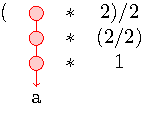
\includegraphics[scale=1.6]{../fig/sharing.pdf}
        \caption{Sharing bei einer Liste von Ausdrücken}
        \label{fig:sharing}
    \end{figure}
    \end{minipage}
    \begin{minipage}[c]{0.5\linewidth}
    \begin{figure}[H]
        \centering
        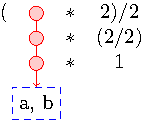
\includegraphics[scale=1.6]{../fig/classes.pdf}
        \caption{Kombination aus Sharing und Klassen bei einer Liste von Ausdrücken}
        \label{fig:classes}
    \end{figure}
\end{minipage}}

Auf den beiden vorgestellten Prinzipien fußen auch \textit{E-Graphs}. \textit{E-Graphs} bestehen aus zwei Komponenten: \textit{E-Classes} und \textit{E-Nodes}. 
Abbildung~\ref{fig:egraphexp} zeigt einen beispielhaften E-Graph. \textit{E-Nodes} sind dabei weiß und \textit{E-Classes} beige eingefärbt.

\begin{figure}[H]
  \centering
  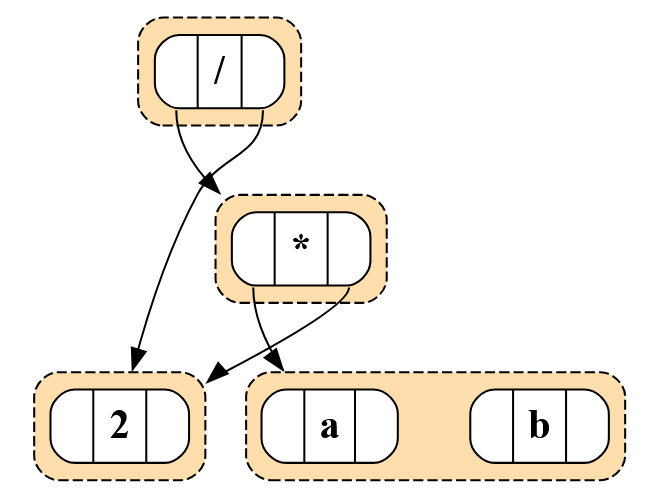
\includegraphics[scale=0.5]{../fig/egraph_exp.png}
  \caption{Beispiel eines E-Graphs, der die Ausdrücke $(a * 2) / 2$ und $(b * 2) / 2$ enthält}
  \label{fig:egraphexp}
\end{figure}

\textit{E-Nodes} sind Knoten (ähnlich zum Element $a$ in Abbildung~\ref{fig:sharing}), die arithmetische Operationen, Zahlen oder Variablen enthalten können.
% Dabei ist zu beachten, dass bei arithmetischen Operationen kein Sharing betrieben wird, da diese auf unterschiedliche  zeigen können.  
Einer \textit{E-Node} werden als Argumente \textit{E-Classes} übergeben. In Beispiel~\ref{fig:egraphexp} wird der \textit{E-Node} $\mathbf{*}$ die 
\textit{E-Class} mit den beiden \textit{E-Nodes} $\mathbf{a}$ und $\mathbf{b}$ und die \textit{E-Class} mit der \textit{E-Node} $\mathbf{2}$ übergeben. 
\textit{E-Classes} stellen also Äquivalenzklassen dar, die äquivalente \textit{E-Nodes} enthalten.

% \textit{E-Classes} sind Äquivalenzklassen mit \textit{E-Nodes}, die äquivalent zueinander sind. 
% Im Beispiel~\ref{fig:egraphexp} sind $a$ und $b$ äquivalent zueinander.
% Als Argumente von \textit{E-Nodes} werden \textit{E-Classes} übergeben.
% Im Beispiel~\ref{fig:egraphexp} wird dem \textit{E-Node} $*$ die \textit{E-Class} mit den beiden \textit{E-Nodes} $a$ und $b$ und die \textit{E-Class} mit dem \textit{E-Node} $2$ übergeben. 
% Es wird also ausgenutzt, dass $a$ und $b$ in der gleichen \textit{E-Class} sind. 

\subsubsection{Implementierung von E-Graphs}

Es gibt verschiedene Ansätze für die Implementierung von \textit{E-Graphs}. Der Ansatz, auf dem diese Arbeit beruht, ist eine Kombination aus zwei Quellen 
(siehe verwandte Arbeiten~\ref{sub:verwandtearbeiten}).
Ein \textbf{E-Graph} wird nach~\cite{2021-egg} als Tuple $(\mathbf{U}, \mathbf{M}, \mathbf{H})$ mit folgenden Eigenschaften definiert:

\begin{itemize}
  \item $\mathbf{U}$ Eine Union-Find-Datenstruktur, die eine Äquivalenzrelation über IDs abspeichert.
  \item $\mathbf{M}$ Eine (Hash)-map, die IDs von E-Classes auf E-Classes abbildet. 
  \item $\mathbf{H}$ Eine (Hash)-map, die E-Nodes auf IDs von E-Classes abbildet.
\end{itemize}

Der \textit{E-Graph} als Datenstruktur für Beispiel~\ref{fig:egraphexp} würde also wie folgt aussehen:

\begin{itemize}
  \item $\mathbf{U}$: \{ID1\}, \{ID2\}, \{ID3\}, \{ID4, ID5\} 
  \item $\mathbf{M}$: $ID1 \rightarrow EClass(\ldots)$, $ID2 \rightarrow EClass(\ldots)$, $ID3 \rightarrow EClass(\ldots)$, \ldots 
  \item $\mathbf{H}$: $/ \rightarrow ID1$, $* \rightarrow ID2$, $2 \rightarrow ID3$, $a \rightarrow ID4$, $b \rightarrow ID5$
\end{itemize}

\subsection{Equality Saturation}

Nachdem \textit{E-Graphs} eingeführt wurden stellt sich jetzt die Frage, wie damit ein optimaler Ausdruck gefunden werden kann.
Hierzu kann die Methode der \textit{Equality Saturation} eingesetzt werden.
\textit{Equality Saturation} beschreibt eine aus zwei Phasen bestehende, iterative Methode.
In der ersten Phase werden \textit{rewrite rules} auf den \textit{E-Graph} angewendet, bis sich keine Änderungen an diesem mehr ergeben.
Der E-Graph gilt nach dieser Phase als \textit{saturiert}.
In der zweiten Phase kann mithilfe einer Kostenfunktion der optimale Ausdruck aus dem E-Graph extrahiert werden.
Algorithmus~\ref{alg:eqsat} zeigt den Prozess der \textit{Equality Saturation}.

\begin{algorithm}[H]
  \caption{Traditioneller Equality Saturation Workflow nach~\cite{2021-egg}}\label{alg:eqsat}
  \begin{algorithmic}
    \Function{eqsat}{expr, rewrites}
    \State egraph $\gets$ initial\_egraph(expr)
    
    \While{$\mathbf{not}$ egraph.is\_saturated\_or\_timeout()}
      
      \For{rw in rewrites}
        \For{(subst, eclass) $\mathbf{in}$ egraph.ematch(rw.lhs)}
          \State  eclass2 $\gets$ egraph.add(rw.rhs.subst(subst))
          \State egraph.merge(eclass, eclass2)
        \EndFor 
      \EndFor
    \EndWhile

    \State \Return egraph.extract\_best()
    \EndFunction
  \end{algorithmic}
\end{algorithm}

Mit Algorithmus~\ref{alg:eqsat} gibt es nun eine effiziente Lösung, mit der das \textit{Phase Ordering Problem} umgangen und Speicherbedarf gesenkt werden kann.
Doch auch diese Methode kommt mit einem Haken. Der Extraktionsschritt ist ein NP-schweres Problem~\cite{phaseorder-2009}. In der Praxis ist dennoch möglich ein optimales
Ergebnis in kurzer Zeit zu erhalten, wie die Bibliothek \textit{egg} demonstriert.  
